%%%%%%%%%%%%%%%%%%%%%%%%%%%%%%%%%%%%%%%%%%%%%%%%%%%%%%%%%%%%%%%%%%%%%%%%%%%
%                                                                         %
%                         Introduction to Scintillation                   %
%                                                                         %
%%%%%%%%%%%%%%%%%%%%%%%%%%%%%%%%%%%%%%%%%%%%%%%%%%%%%%%%%%%%%%%%%%%%%%%%%%%
Scintillation detectors (the detectors on which this work is based) utilize a scintillator to convert ionizing radiation into photons, and then transporting and capturing those the emitted photons, commonly with a photomultiplier tube (PMT).
The electrical signal from the PMT is then an indicator of a radiation event in the detector's scintillator material.
The current RPMs with \iso[3]{He} are ion chamber detectors, however, the proposed \iso[6]{Li} glass detectors and \iso[6]{LiF} doped ZnS:Ag detectors are scintillation based detectors. 

\subsection{Organic Scintillators}
An organic scintillator generally has a $\pi$-electron structure, as shown in \autoref{fig:pielectron}.
An incoming electron (liberated from the energy deposition of the ionizing radiation) then excites one of the modes of the $\pi$-electron structure.
Higher singlet states rapidly (on the order of picoseconds) relax to the first singlet state, and excessive vibrational energy (populations of the vibrational sates) is lost.
Thus, after a short period of time the entire excitation population is in the $S_10$ state, and the decay of this state creates the prompt fluorescence.
\begin{figure}
  \centering
  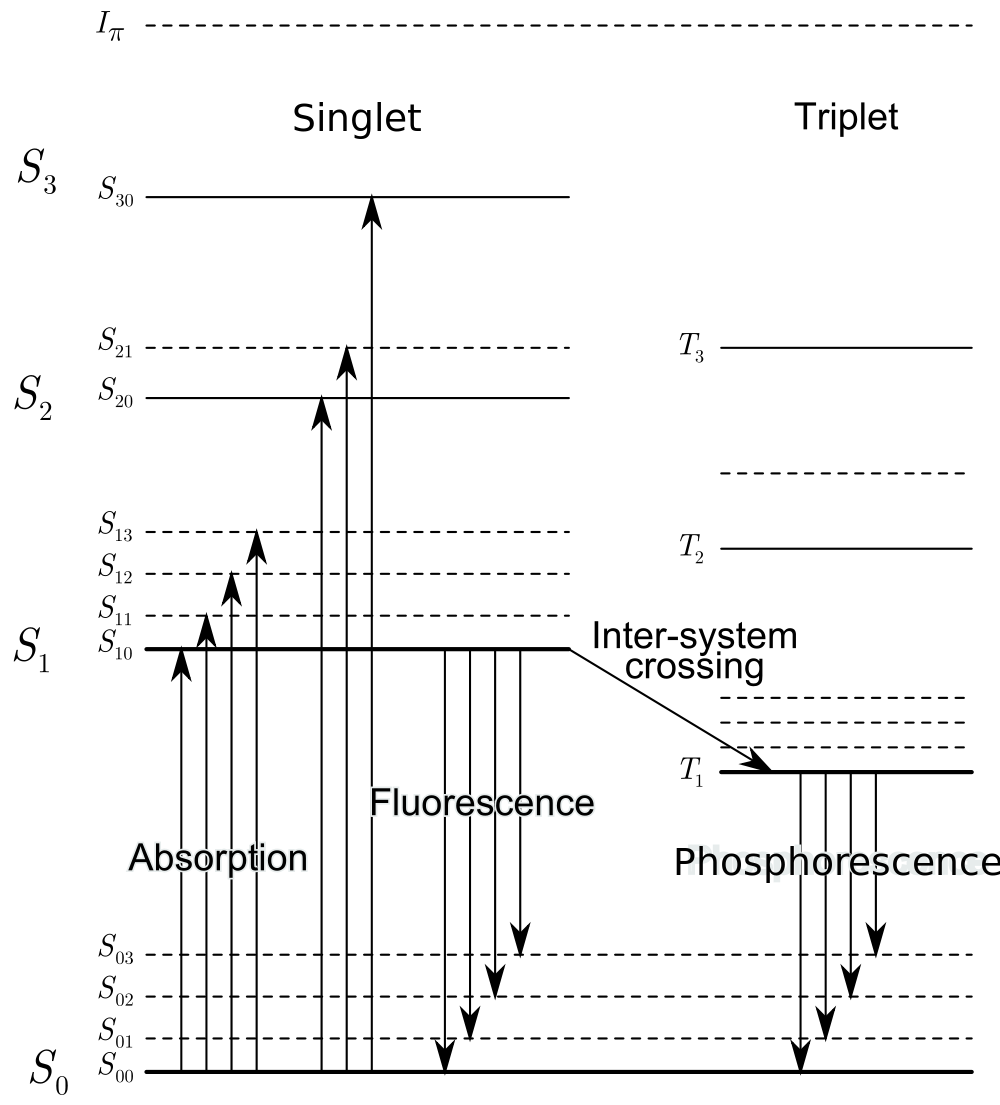
\includegraphics[width=0.6\textwidth]{PiElectronSates}
  \caption[$\pi$ Electron Structure]{Typical $\pi$-electron structure of an organic molecule. The ground state of the molecule is shown as $S_0$, and excited single states are $S_1$, $S_2$ etc The triplet states are $T_1$, $T_2$, with the vibrational states as $S_OO$, $S_01$, $S_02$ and so forth. Figure from Wikipedia.}
  \label{fig:pielectron}
\end{figure}
The excitations of triplet states typically yield delayed scintillation events or phosphorescence.
An excited triplet states immediately decays to the $T_0$ state by internal degradation without a photon emission.
The $T_0$ state typically decays by interacting with another $T_0$ state in a $T_0 + T_0 \to S^* + S_0 + h\nu$ transition.
The excited singlet state $S^*$ then also decays to the $S_0$ state.
The $T_0 + T_0$ transitions is slower than direct singlet state de-excitations, and results in a slow component of the pulse, which can be used for pulse shape discrimination.

The light output of an organic scintillator can be empirically related to the energy deposition in the scintillator through the Birks equation.
In the absence of any quenching it is assumed that the light output per unit length is directly proportional to the energy deposition per unit length \eqref{eqn:LONoQuench}
\begin{align}
  \label{eqn:LONoQuench}
    \frac{dL}{dx} = S_B\frac{dE}{dx}
\end{align}
where \definevar{$S_B$}{absolute scintillation efficiency}.
If quenching of the light from molecules damaged by the radiation is also assumed to be proportional to the energy deposition per track length, than the Birks equation can be written as \eqref{eqn:BirksEquation}
\begin{align}
  \label{eqn:BirksEquation}
    \frac{dL}{dx} = \frac{S_B\frac{dE}{dx}}{1+kB\frac{dE}{dx}}
    \end{align}
    where \definevar{$S_B$}{absolute scintillation efficiency},\definevar{$\frac{dE}{dx}$}{linear stopping power} and \definevar{$kB$}{Birks parameter}, which accounts for the quenching of the light.
For low stopping powers (or particles with a very high energy) the light output per unit track length is linear as the quenching term can be neglected.
However, for particles with a large stopping power the light output along the track length becomes saturated by quenching.
This difference in the pulse height accounts for that difference in light output from a \SI{1}{\MeV} electron compared to a \SI{1}{\MeV} alpha.
The \textit{alpha to beta} ratio provides a measure of this effect, and for the GS20 glass is it typically around 0.23.
This effect is critical in the developed detectors are the reaction products of of the \iso[6]{Li} neutron absorption are both heavily charged particles subject to this effect.
Thus, while there is \SI{4.78}{\MeV} of reaction product energy released in the neutron absorption, the low alpha to beta ratio of the material limits the actual number of scintillation events.

\subsection{Pulse Height Deficit}
The concept of alpha to beta ratio is extended for other charged ions as the pulse height deficit.
The pulse height deficit is defined as a measure the apparent energy loss (as seen from the pulse height) of a heavy charged ion compared to an electron.  
The apparent loss in energy of the heavy charged charged ions relative to
This is measured as the difference between the energy of the heavy ion and its apparent energy from the pulse height.  
Several researchers have investigated the light output of scintillators in response to different types of ionizing radiation.
\autoref{fig:lightYieldVerbinski} summarizes the results of \cite{Verbinski_1968} in which the pulse height deficit is apparent for the as the charged ions become heavier.
\begin{figure}
  \centering
  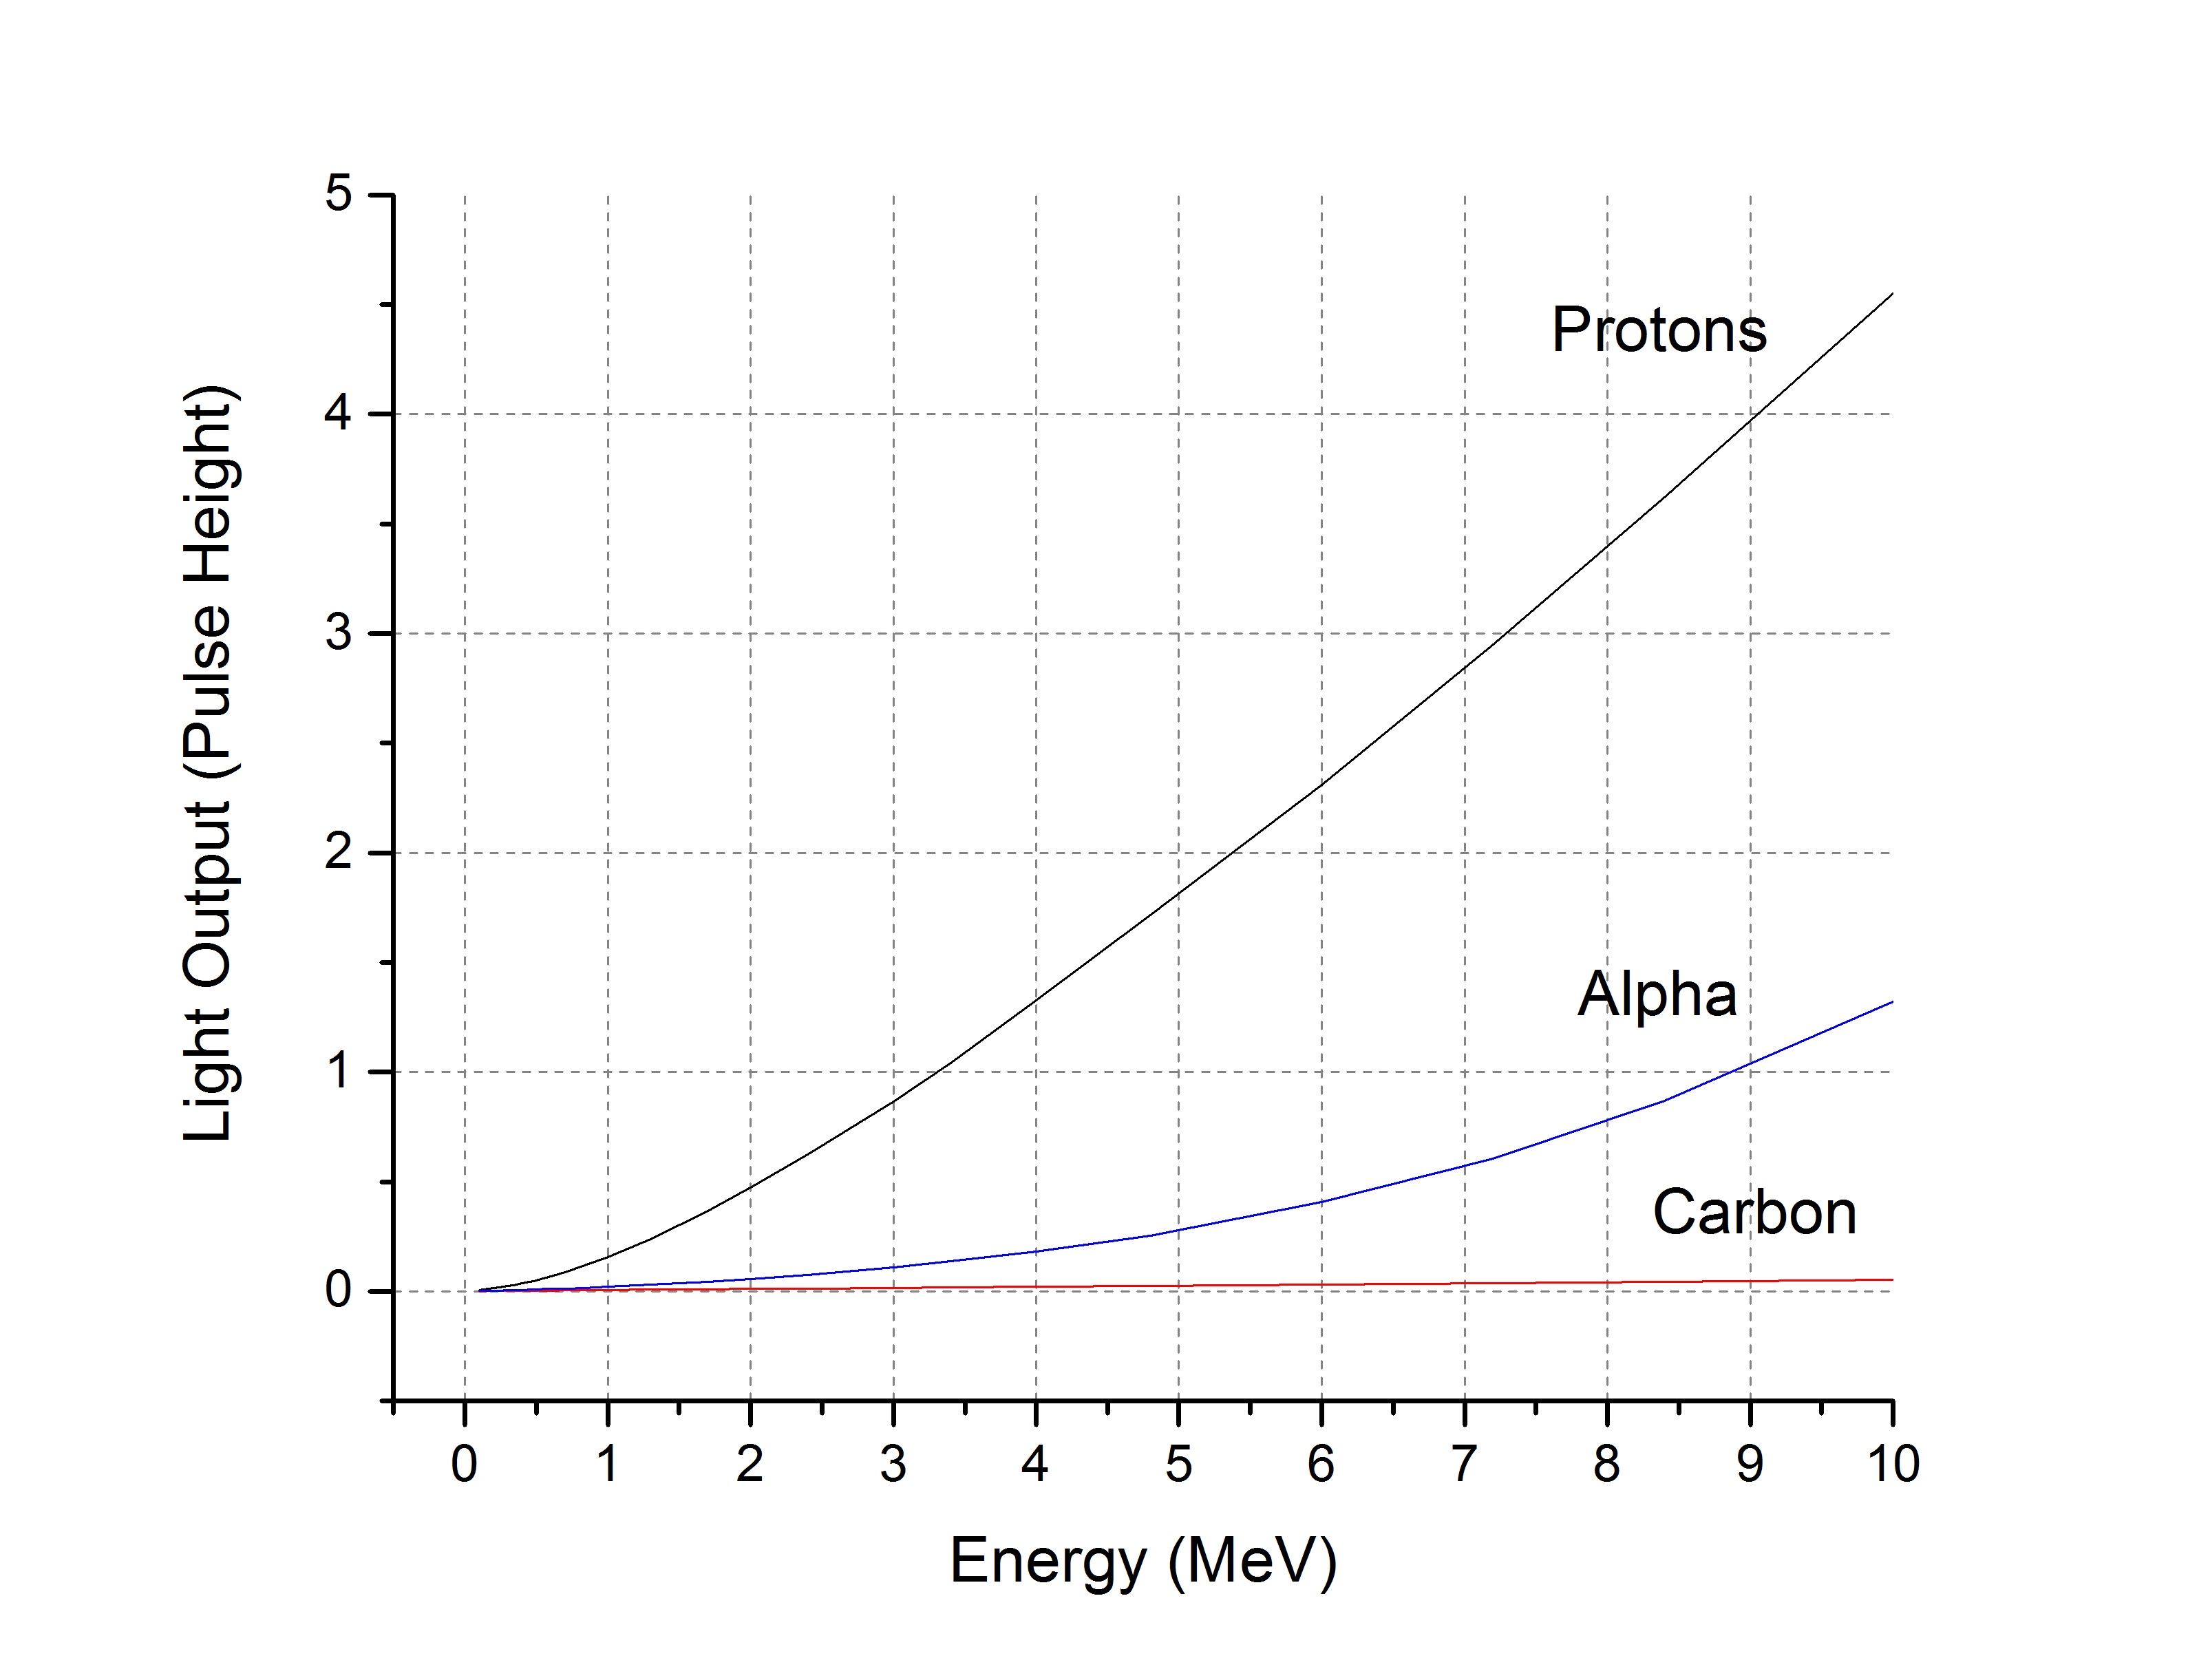
\includegraphics[width=0.6\textwidth]{Verbinski_LightYield_AlpahCarbonProton}
  \caption[Light yield non-proporitonality of anthracene]{Light yield non-proproitonality of antrhacene. Data from \cite{Verbinski_1968}.}
  \label{fig:lightYieldVerbinski}
\end{figure}

An illustration of the energy deposition between the different particles resulting in the pulse height deficit is presented in \autoref{fig:ParticleTracks}.
The electrons, with their low stopping power and broad track structure deposit their energy over a broader range than do the heavy charged ions (which tend to have rather collimated tracks).
Thus, the heavy charged ions deposit a large amount of their energy in a small volume, completely ionizing that volume and inhibiting scintillation.
\begin{figure}
  \begin{subfigure}[b]{0.45\textwidth}
    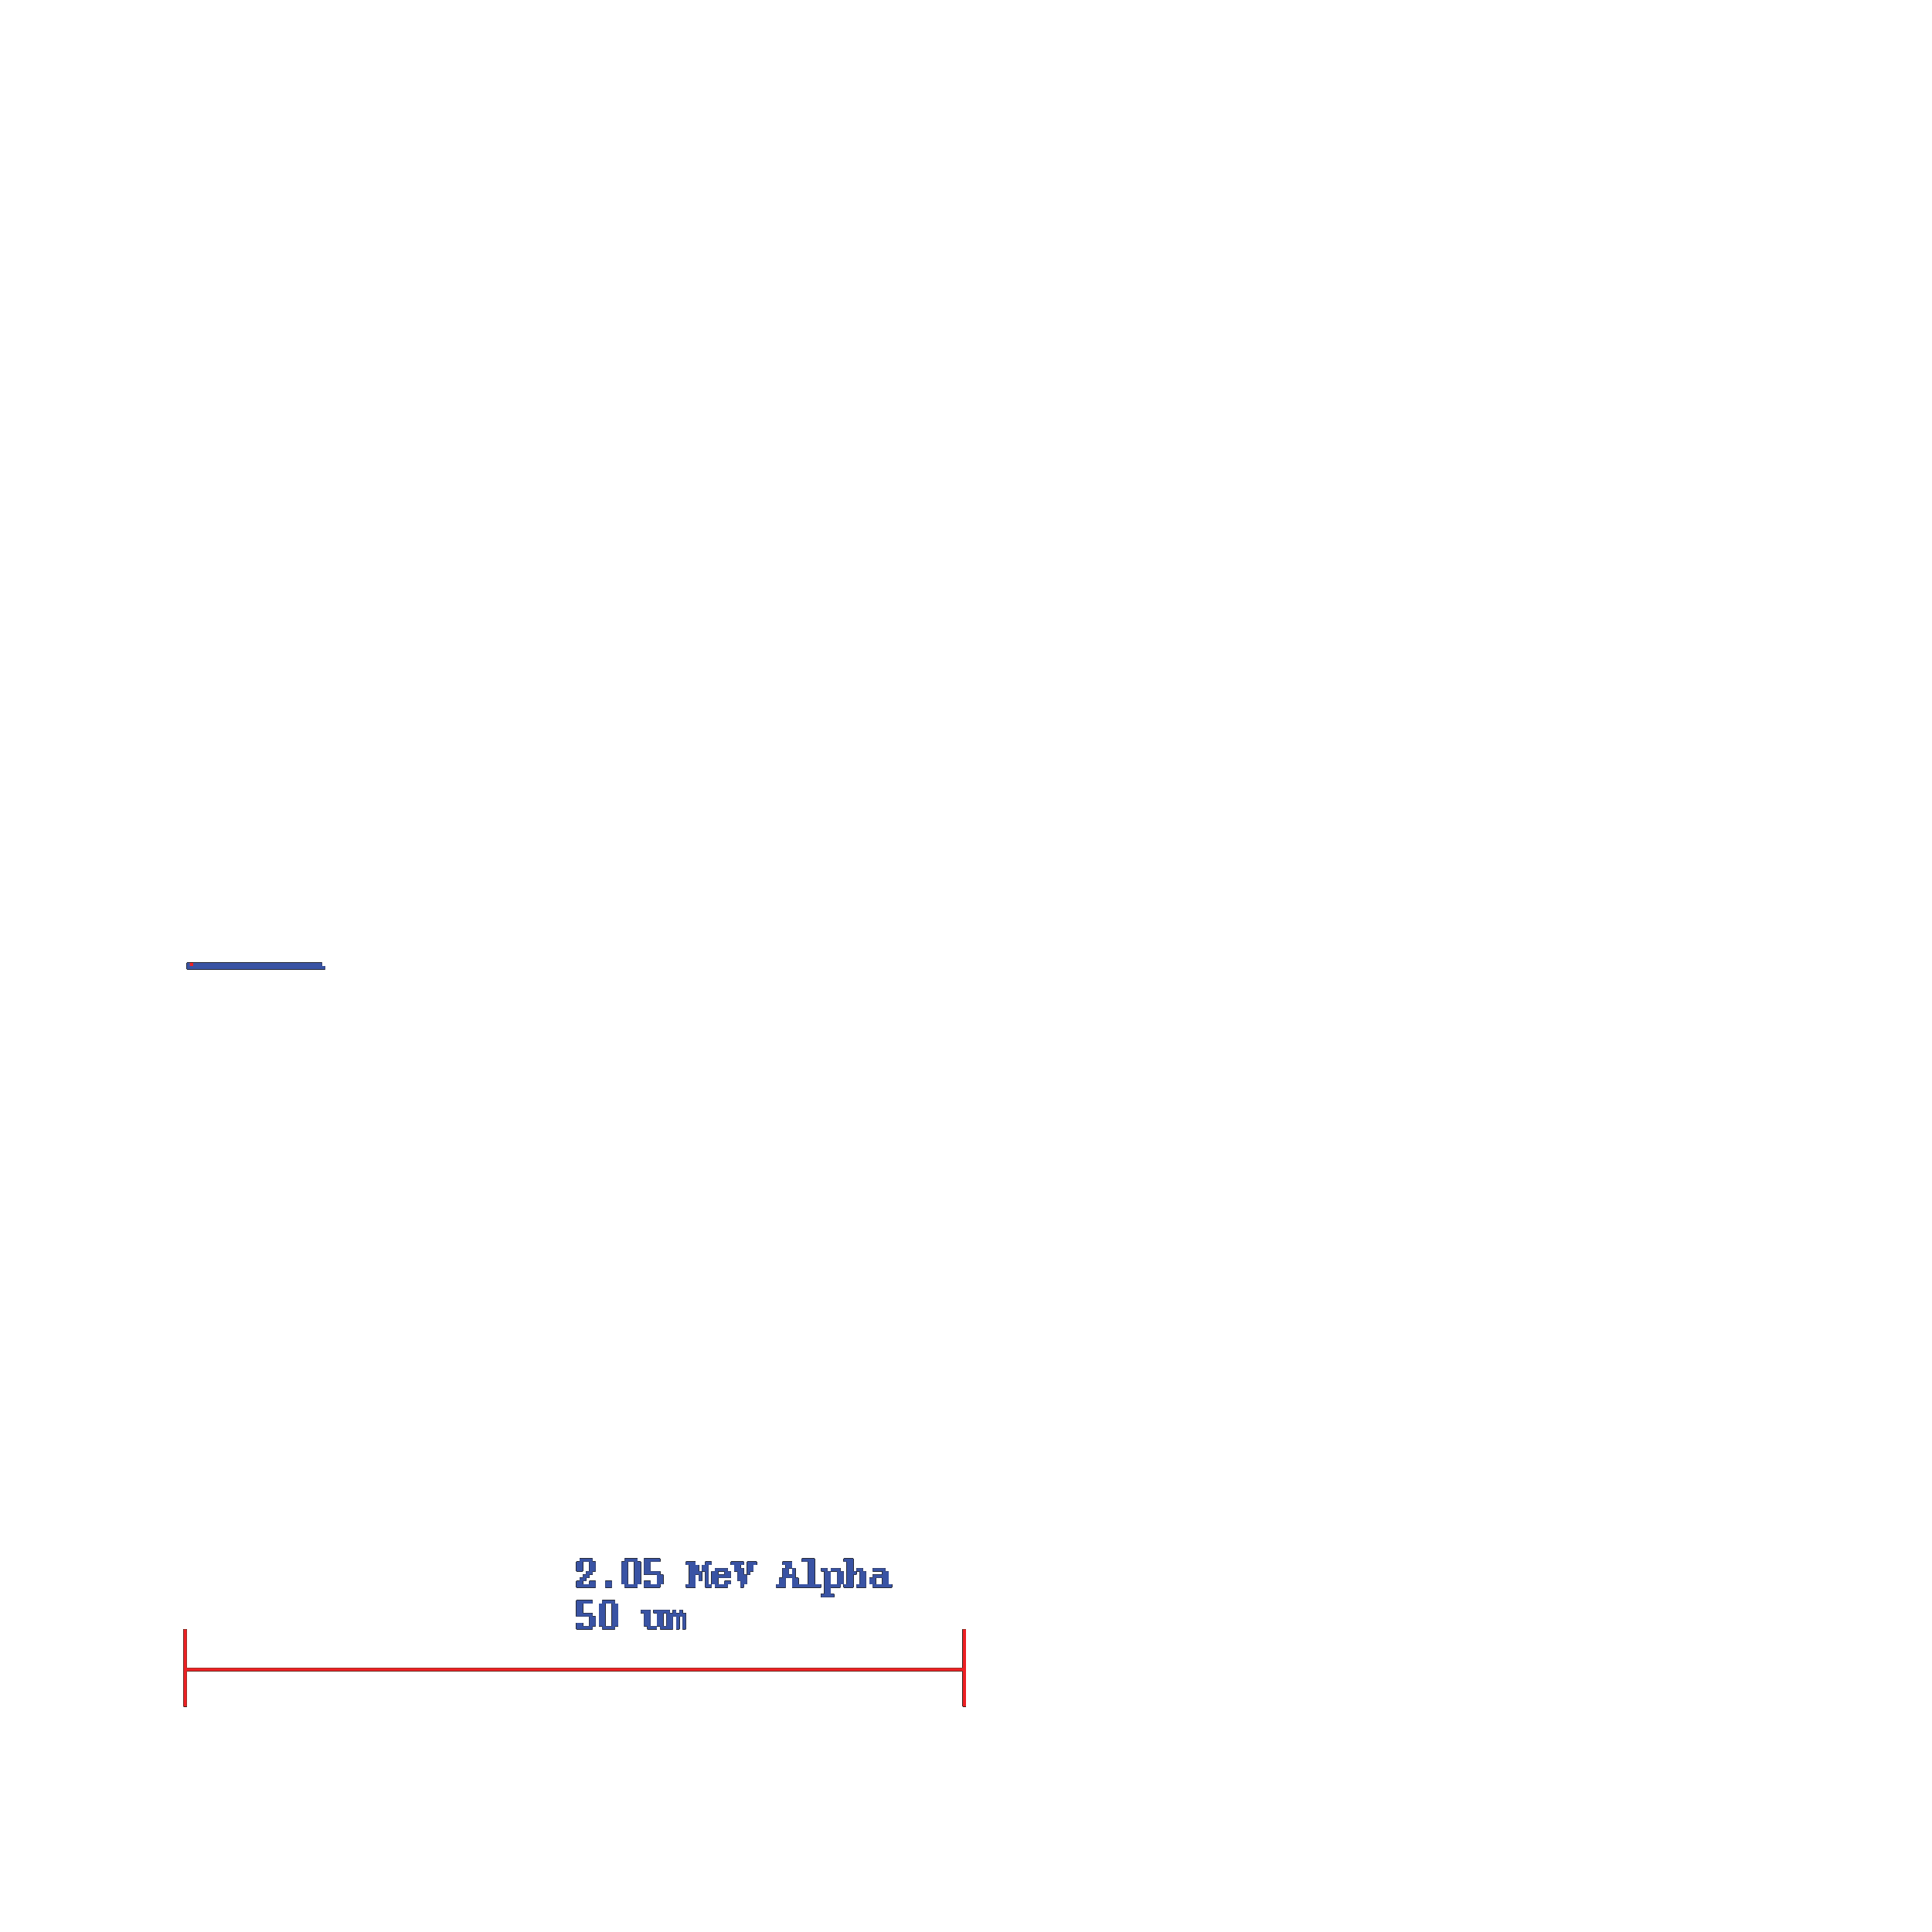
\includegraphics[width=\textwidth]{alphaTrack_0}
    \caption{\SI{2.05}{\MeV} Alpha}
  \end{subfigure}% 
  ~
  \begin{subfigure}[b]{0.45\textwidth}
    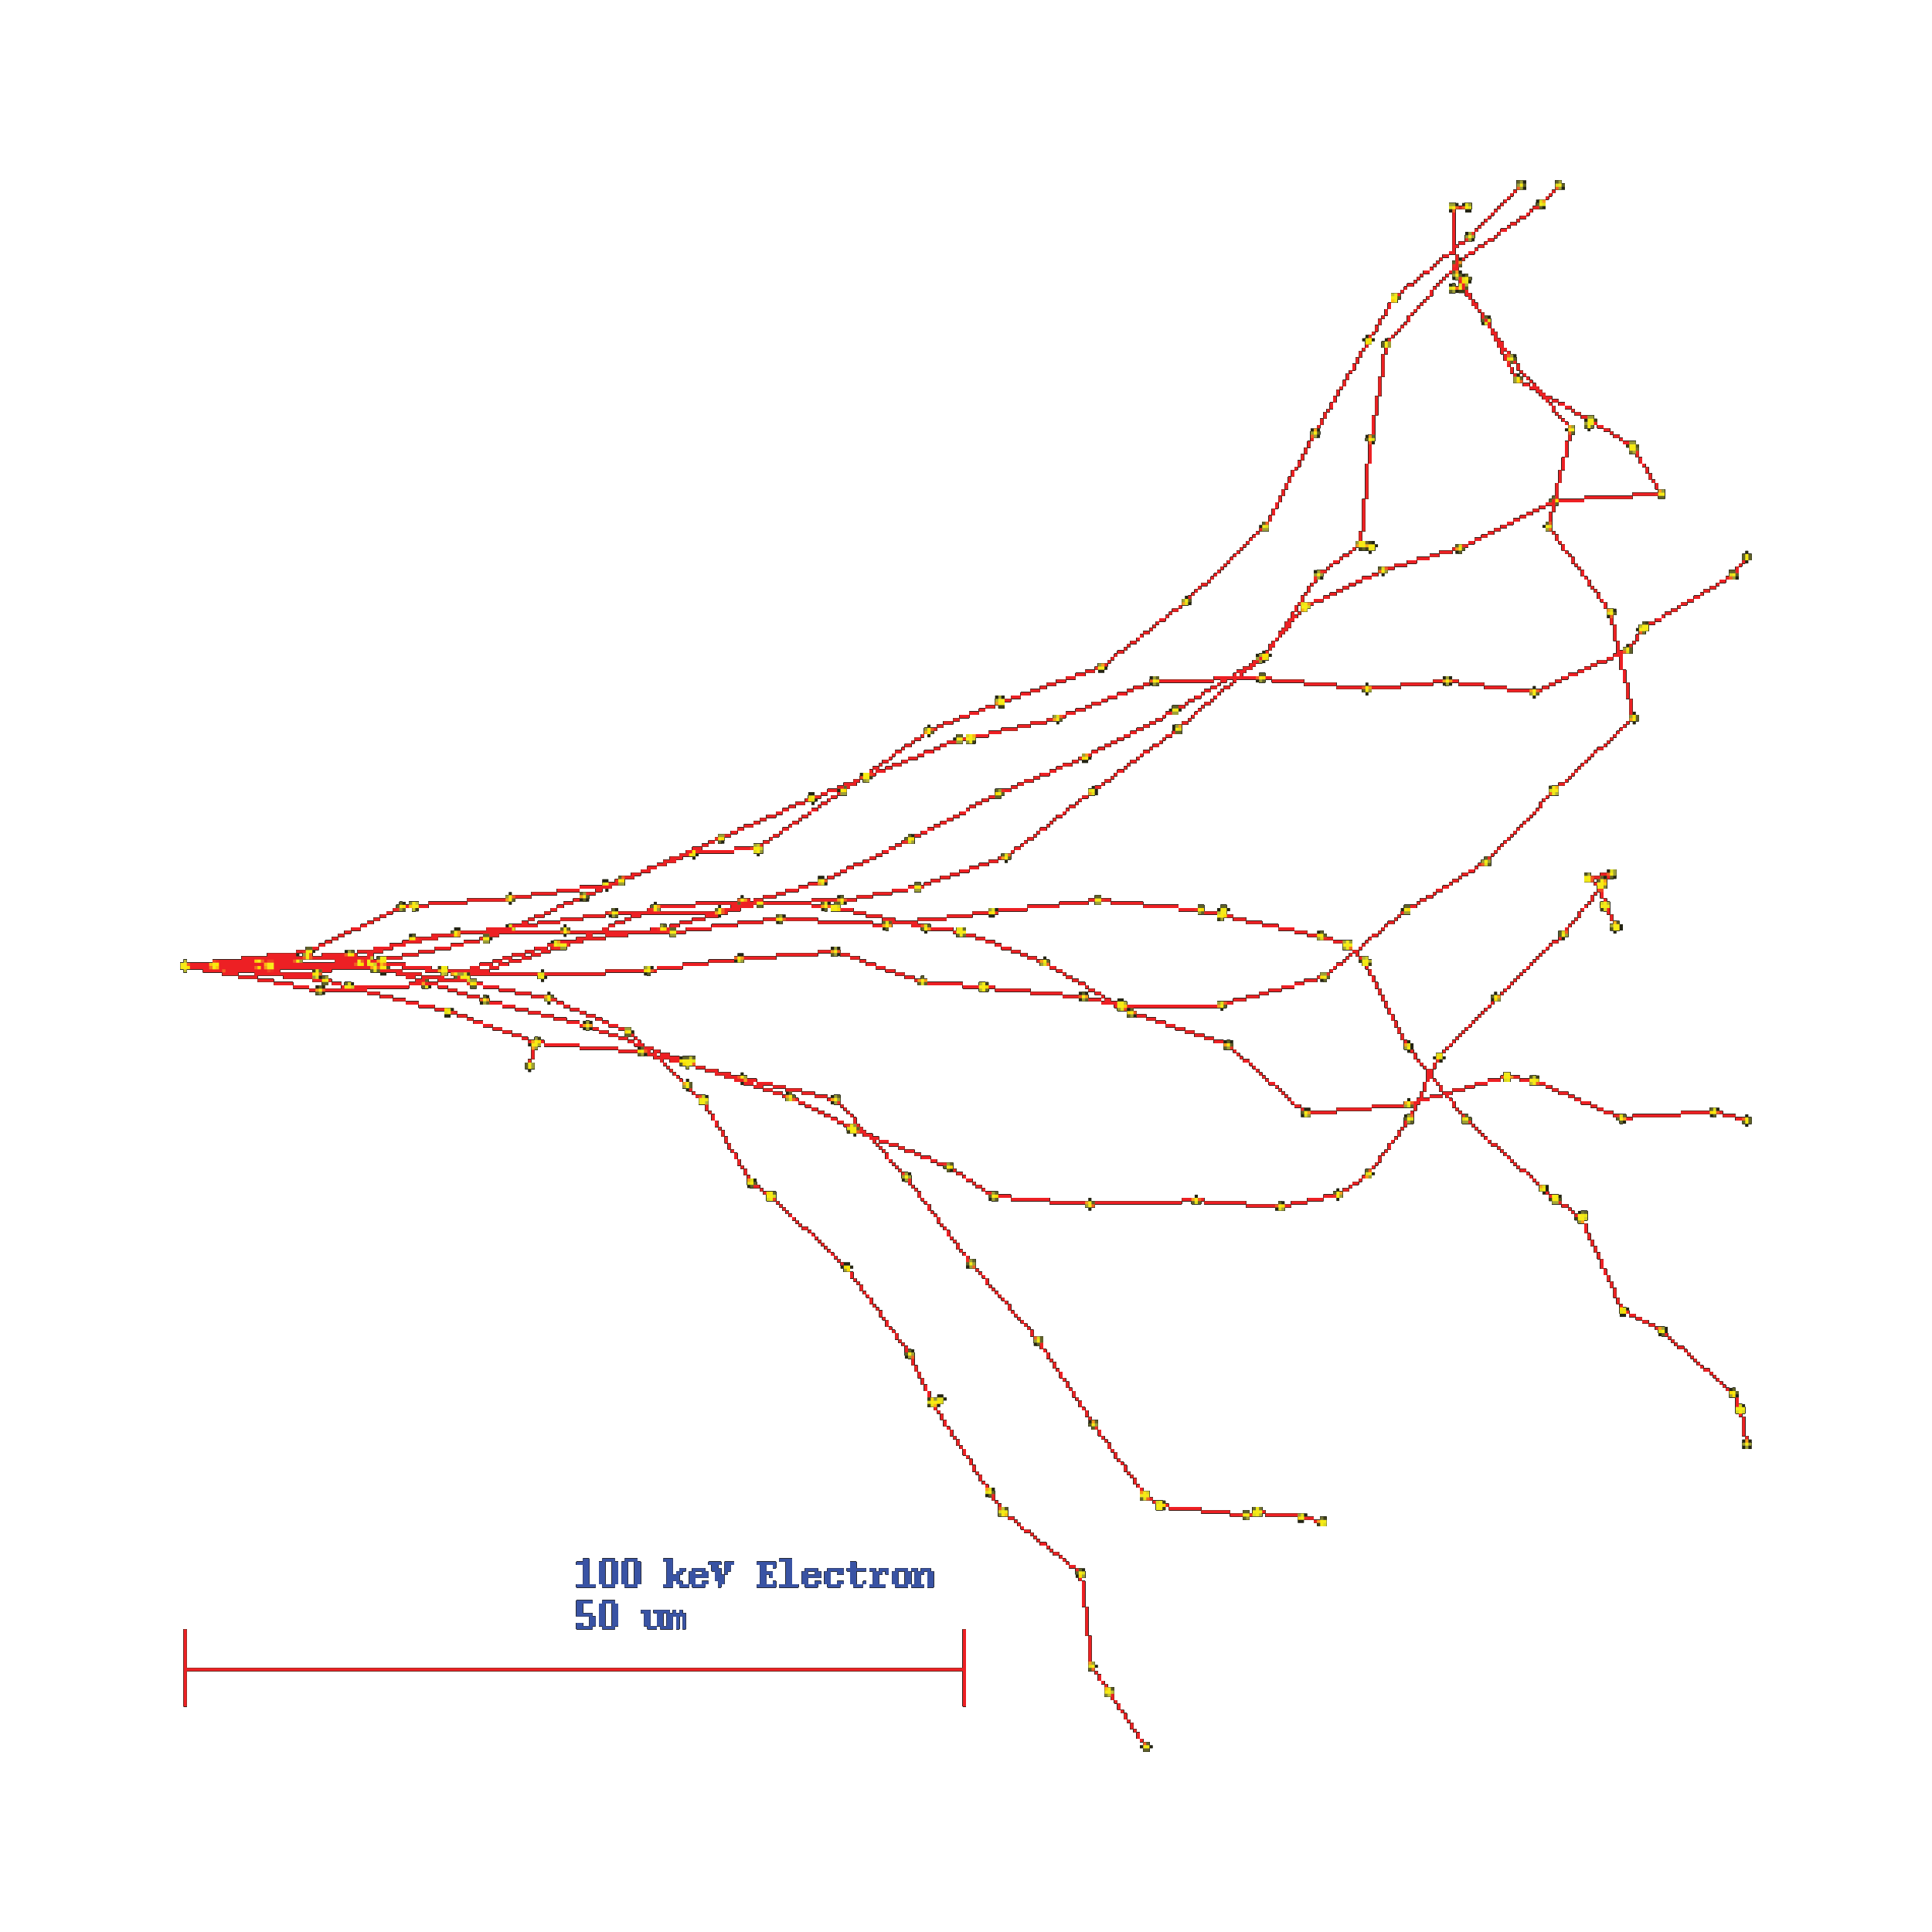
\includegraphics[width=\textwidth]{electronTrack_100keV_0}
    \caption{\SI{100}{\keV} Electron}
  \end{subfigure}
  
  \begin{subfigure}[b]{0.45\textwidth}
    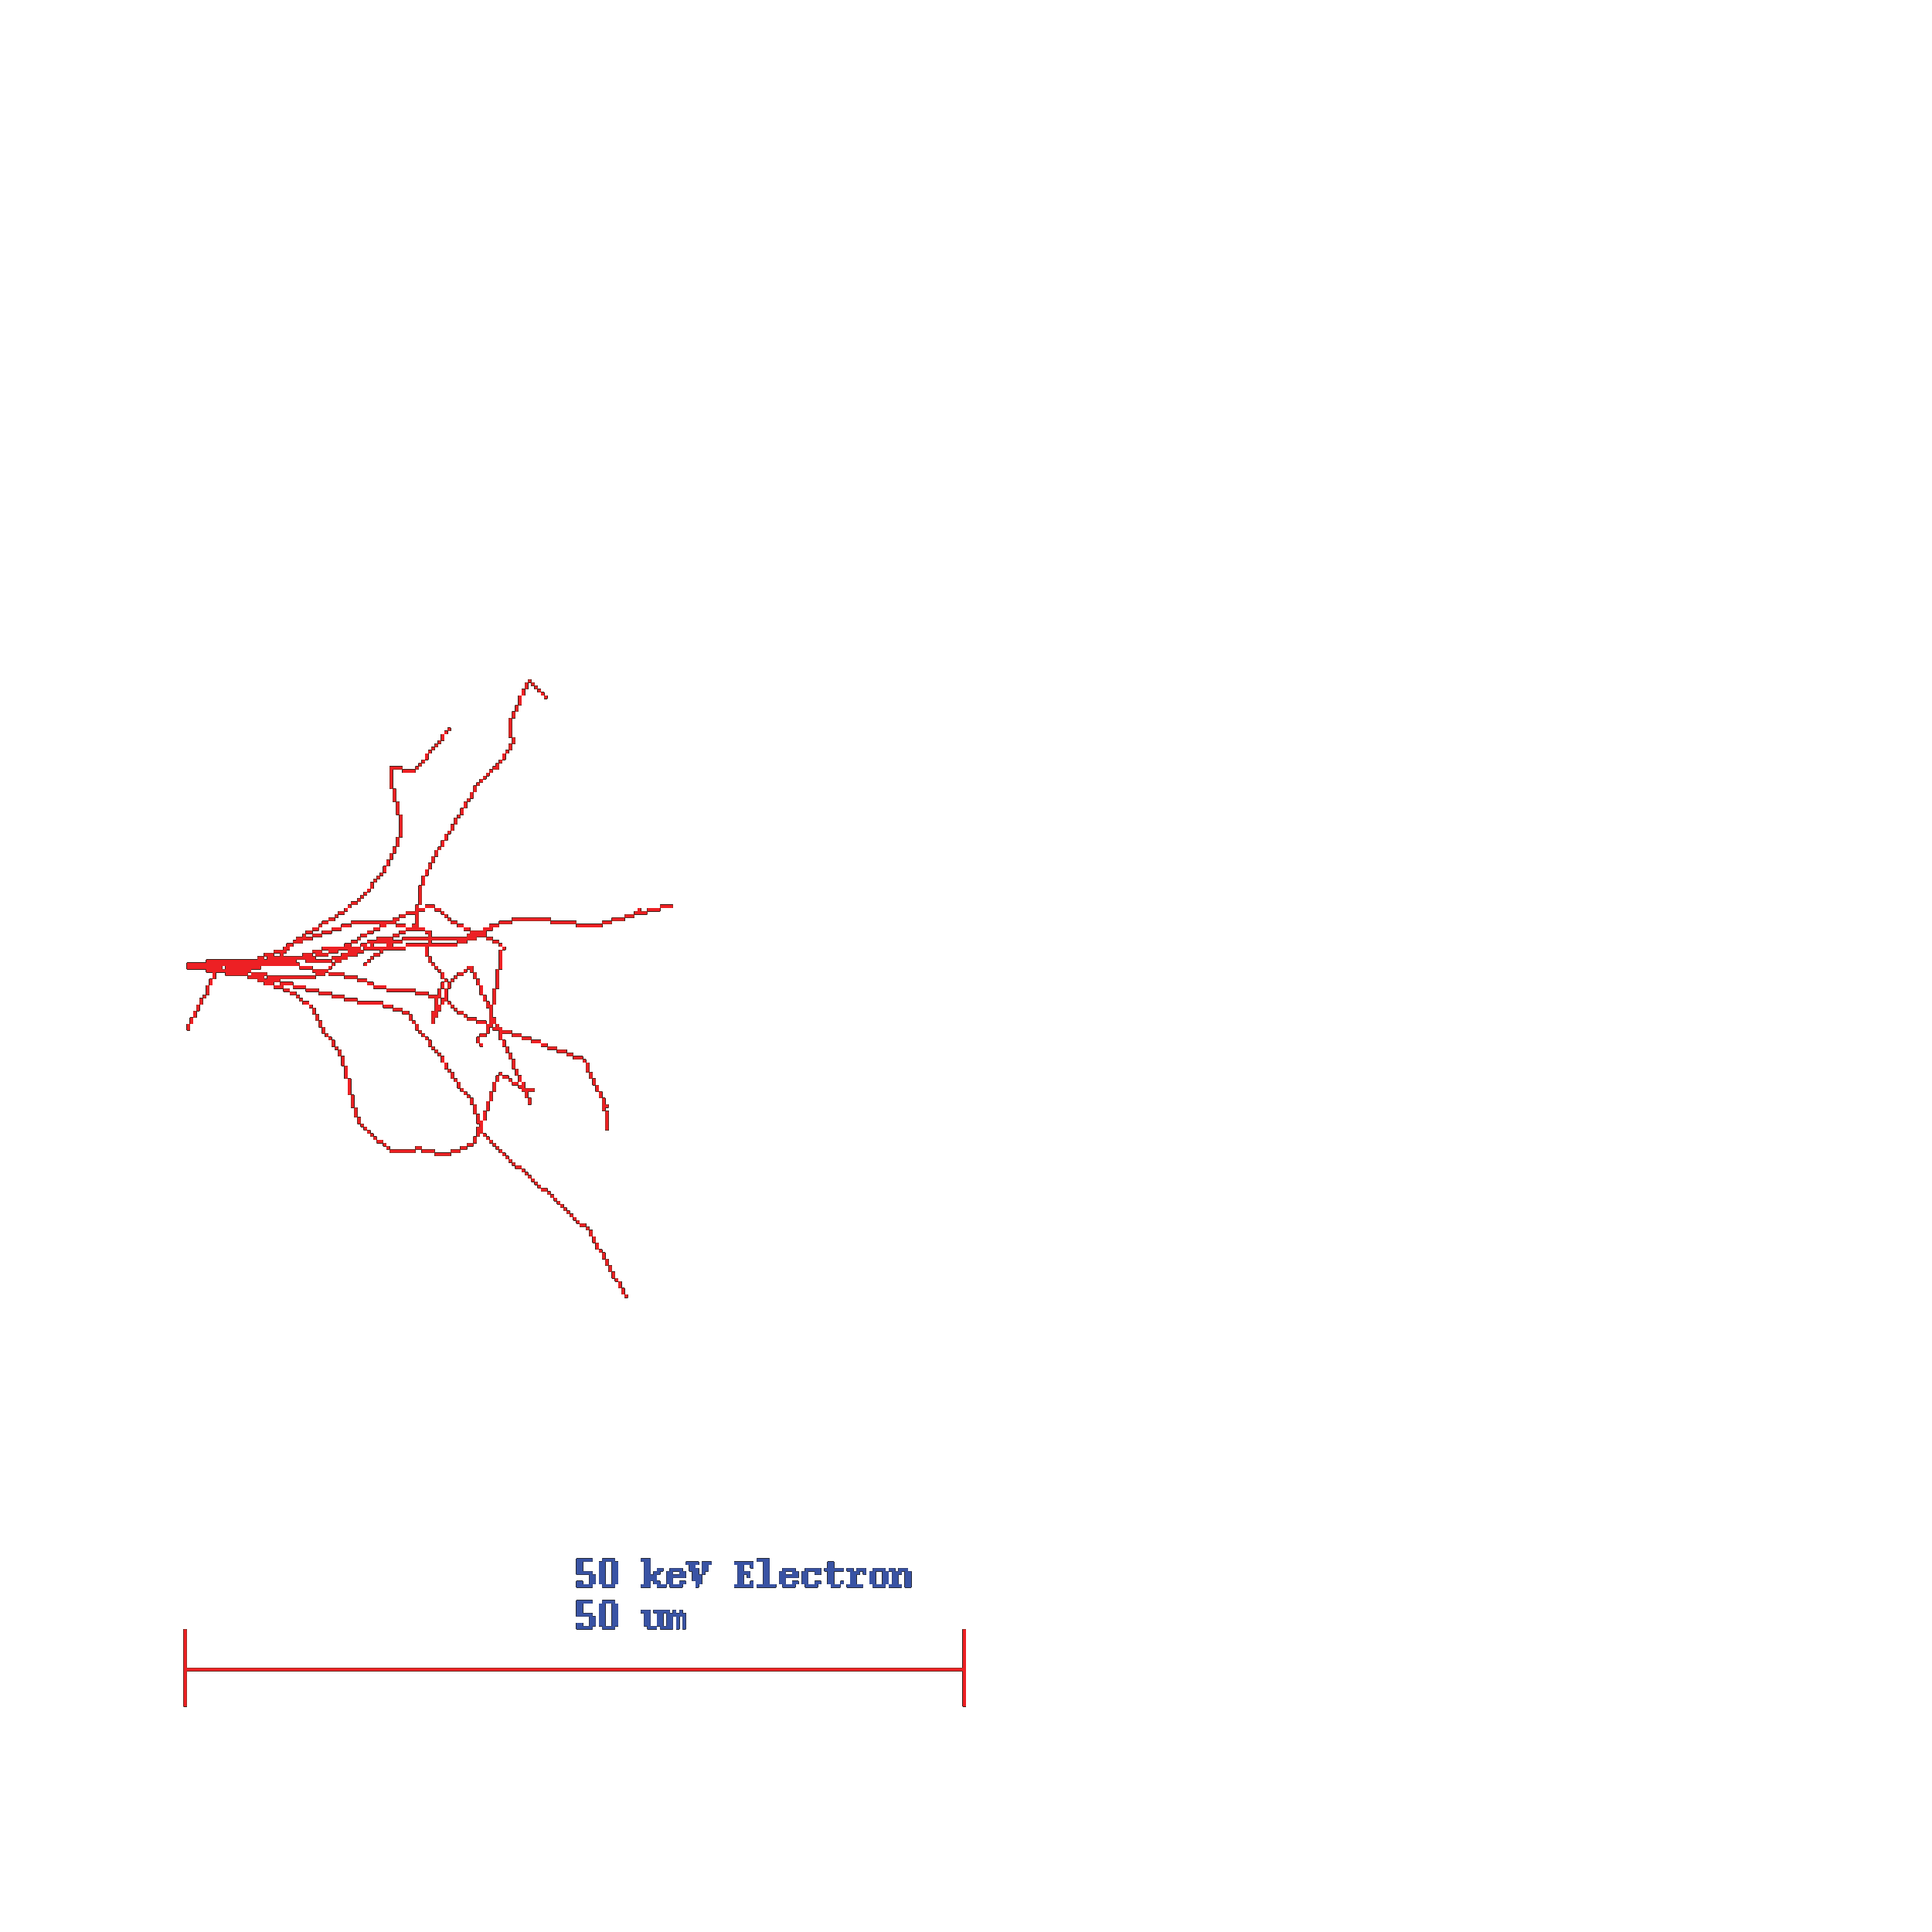
\includegraphics[width=\textwidth]{electronTrack_50keV_0}
    \caption{\SI{50}{\keV} Electron}
  \end{subfigure}%
  ~
  \begin{subfigure}[b]{0.45\textwidth}
    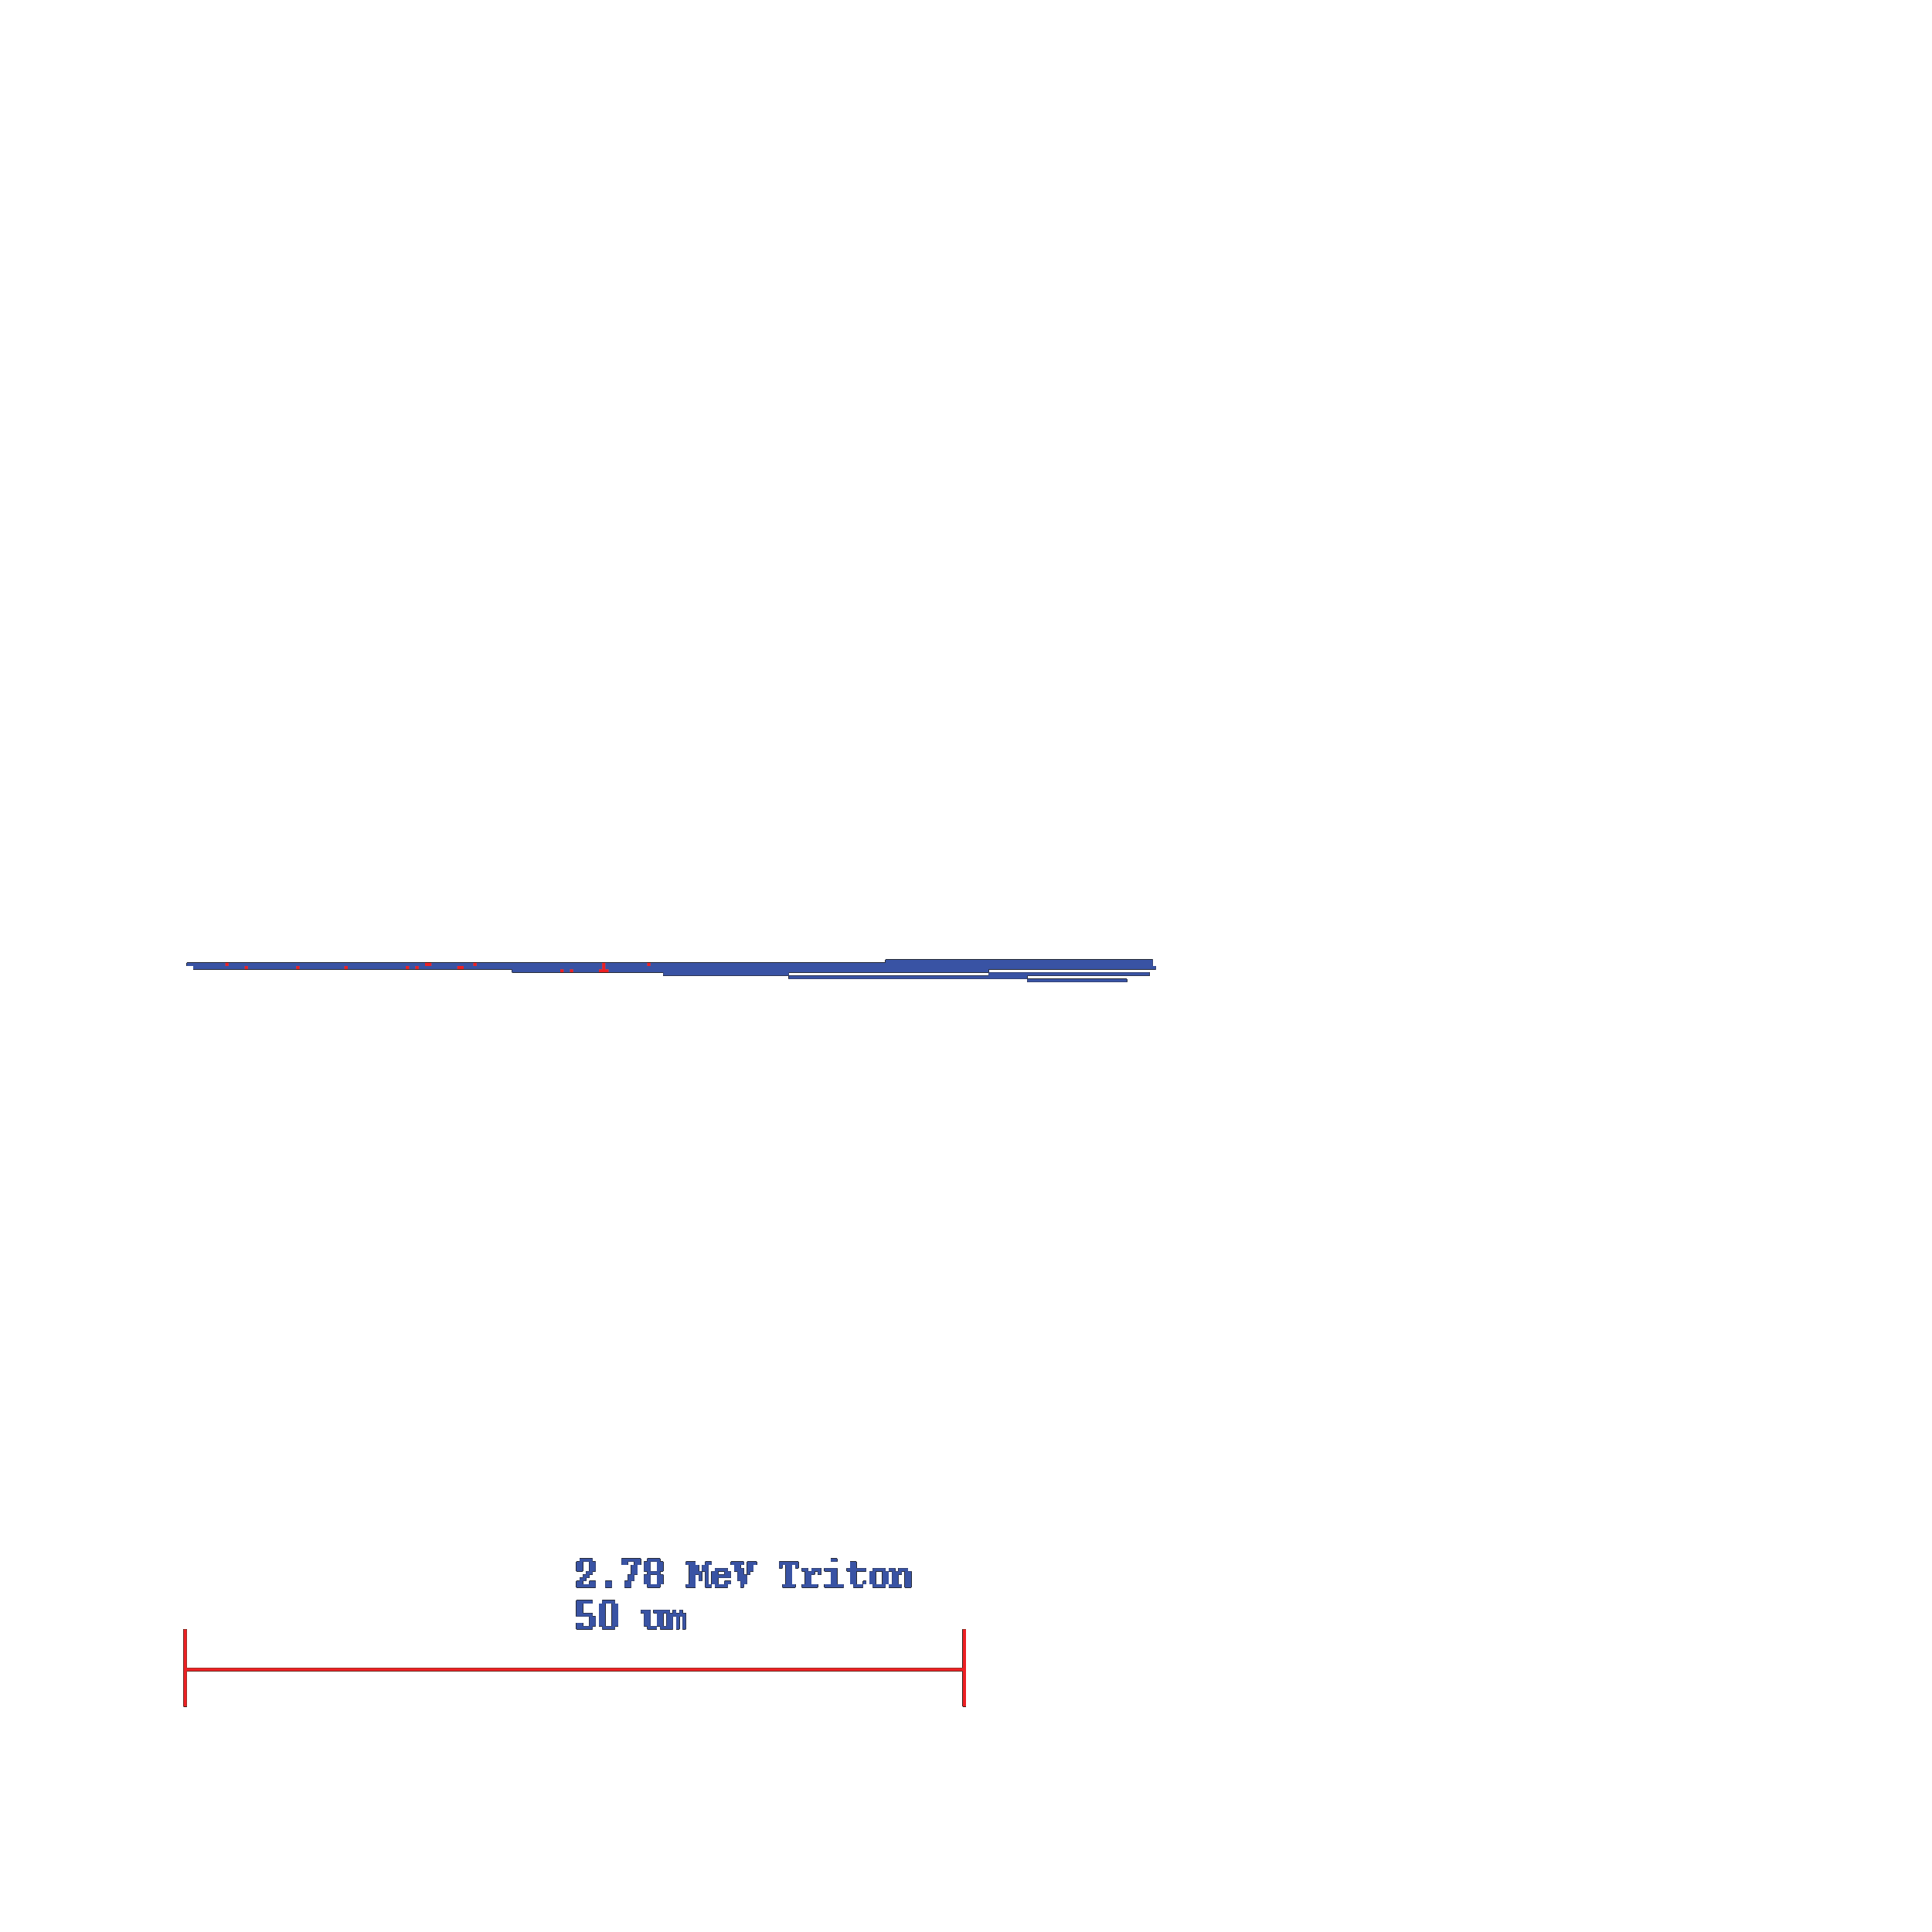
\includegraphics[width=\textwidth]{tritonTrack_0}
    \caption{\SI{2.73}{\MeV} Triton}
  \end{subfigure}
  \caption[Particle Tracks of Alpha, Triton and Electrons]{GEANT4 simulated Particles tracks of a \SI{10}{\keV} electron, \SI{100}{\keV} electron, \SI{2.05}{\MeV} alpha, and \SI{2.73}{\MeV} triton.  The electron tracks are alot broader than the heavy ion tracks, resulting in a greater spread of the energy deposition and less quenching.}
  \label{fig:ParticleTracks}
\end{figure}

For a \iso[6][Li} based portal monitor scintillator the most likely charged particles would be alphas, tritons and electrons.
GEANT4 has the capability to simulate light quenching by setting an appropriate Birks parameter, and \autoref{fig:SimLightOutputQuench} presents GEANT4 simulated photon distributions in polystyrene with a PPO-POPOP fluor and an assumed light yield of 1,000 photons per MeV.
For highly energetic particles the electrons are almost an order of magnitude more efficient at creating light than the tritons, and about 90 times more efficient than the alphas.
However, it is unlikely that many electrons originating from \iso[60]{Co} interactions in the scintillator will have an energy in the \SI{1}{\MeV} range, more likely that they will be in the \SI{100}{\keV} range.
Thus, as shown in \autoref{fig:SimLightOutputQuench} the triton from the \iso[6]{Li} reaction will produce about an factor of five more photons than at \SI{100}{\keV}, and dominates the number of photons produced the the alpha particle.
\begin{figure}
  \centering
    \begin{subfigure}[b]{0.49\textwidth}
    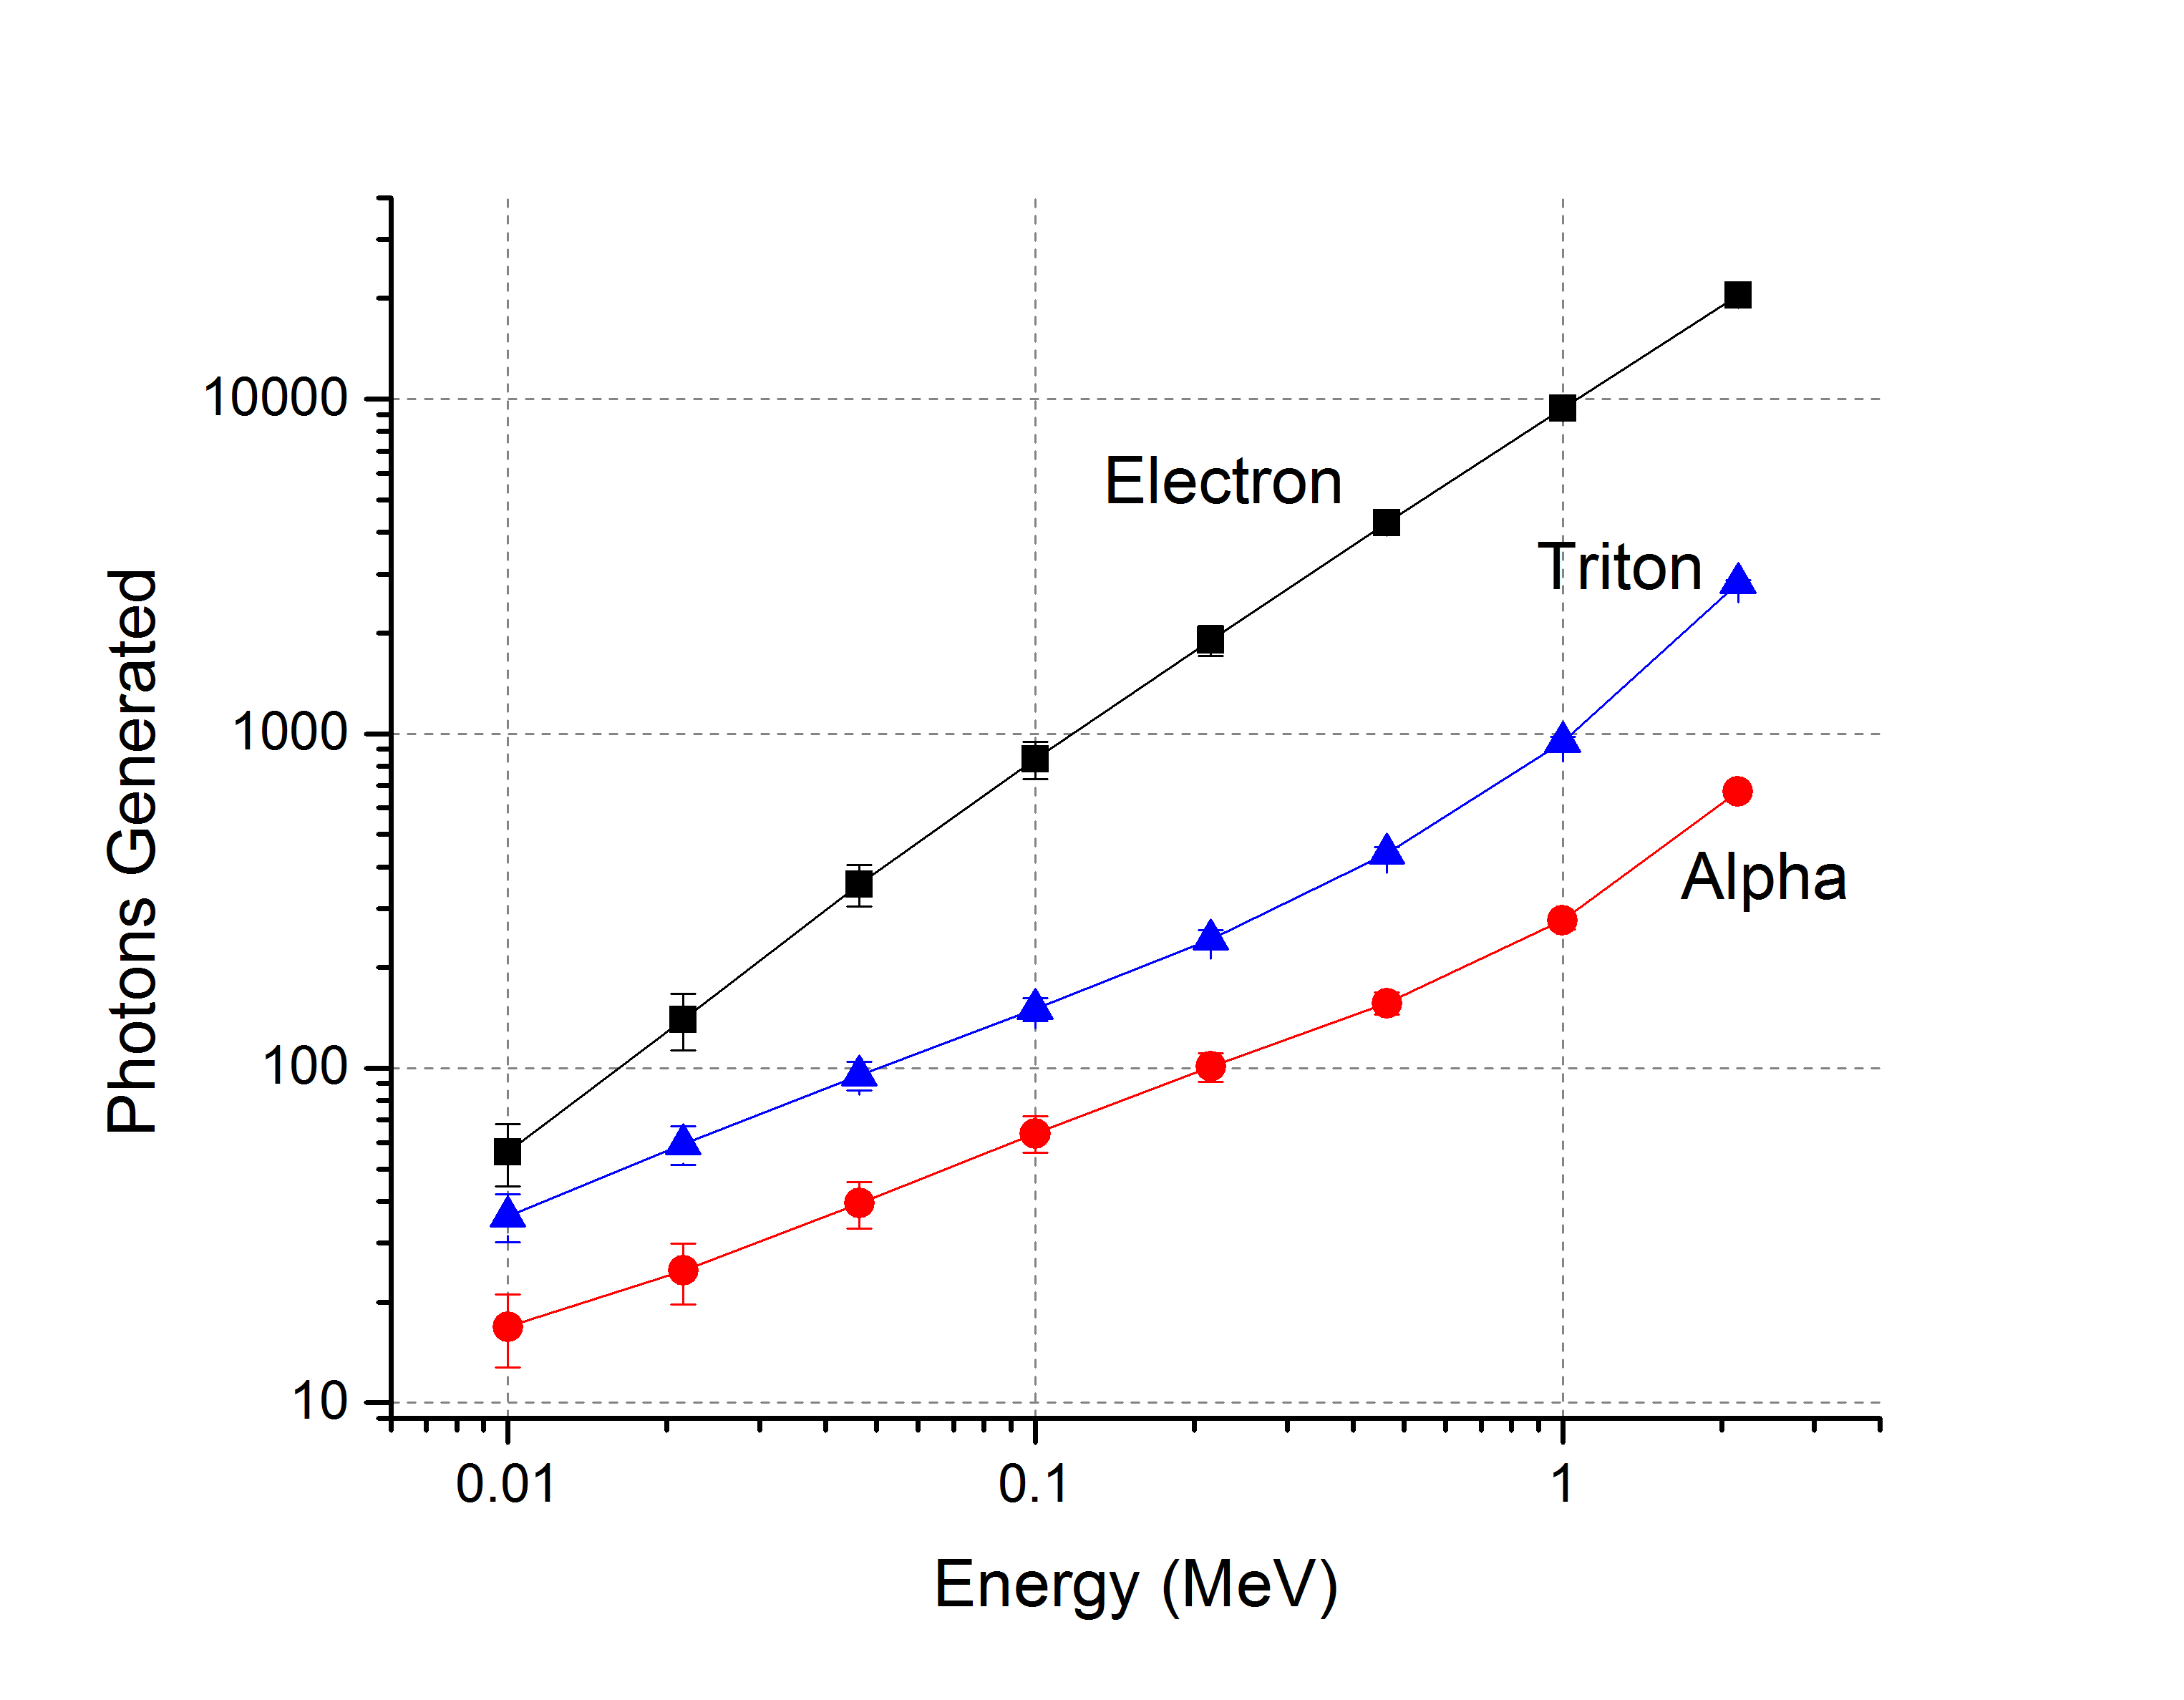
\includegraphics[width=\textwidth]{SimLightQuench}
    \caption{Simulated number of optical photons generated for electrons, alphas, tritons and \iso[7]{Li}.}
  \end{subfigure}%
  ~
  \begin{subfigure}[b]{0.49\textwidth}
    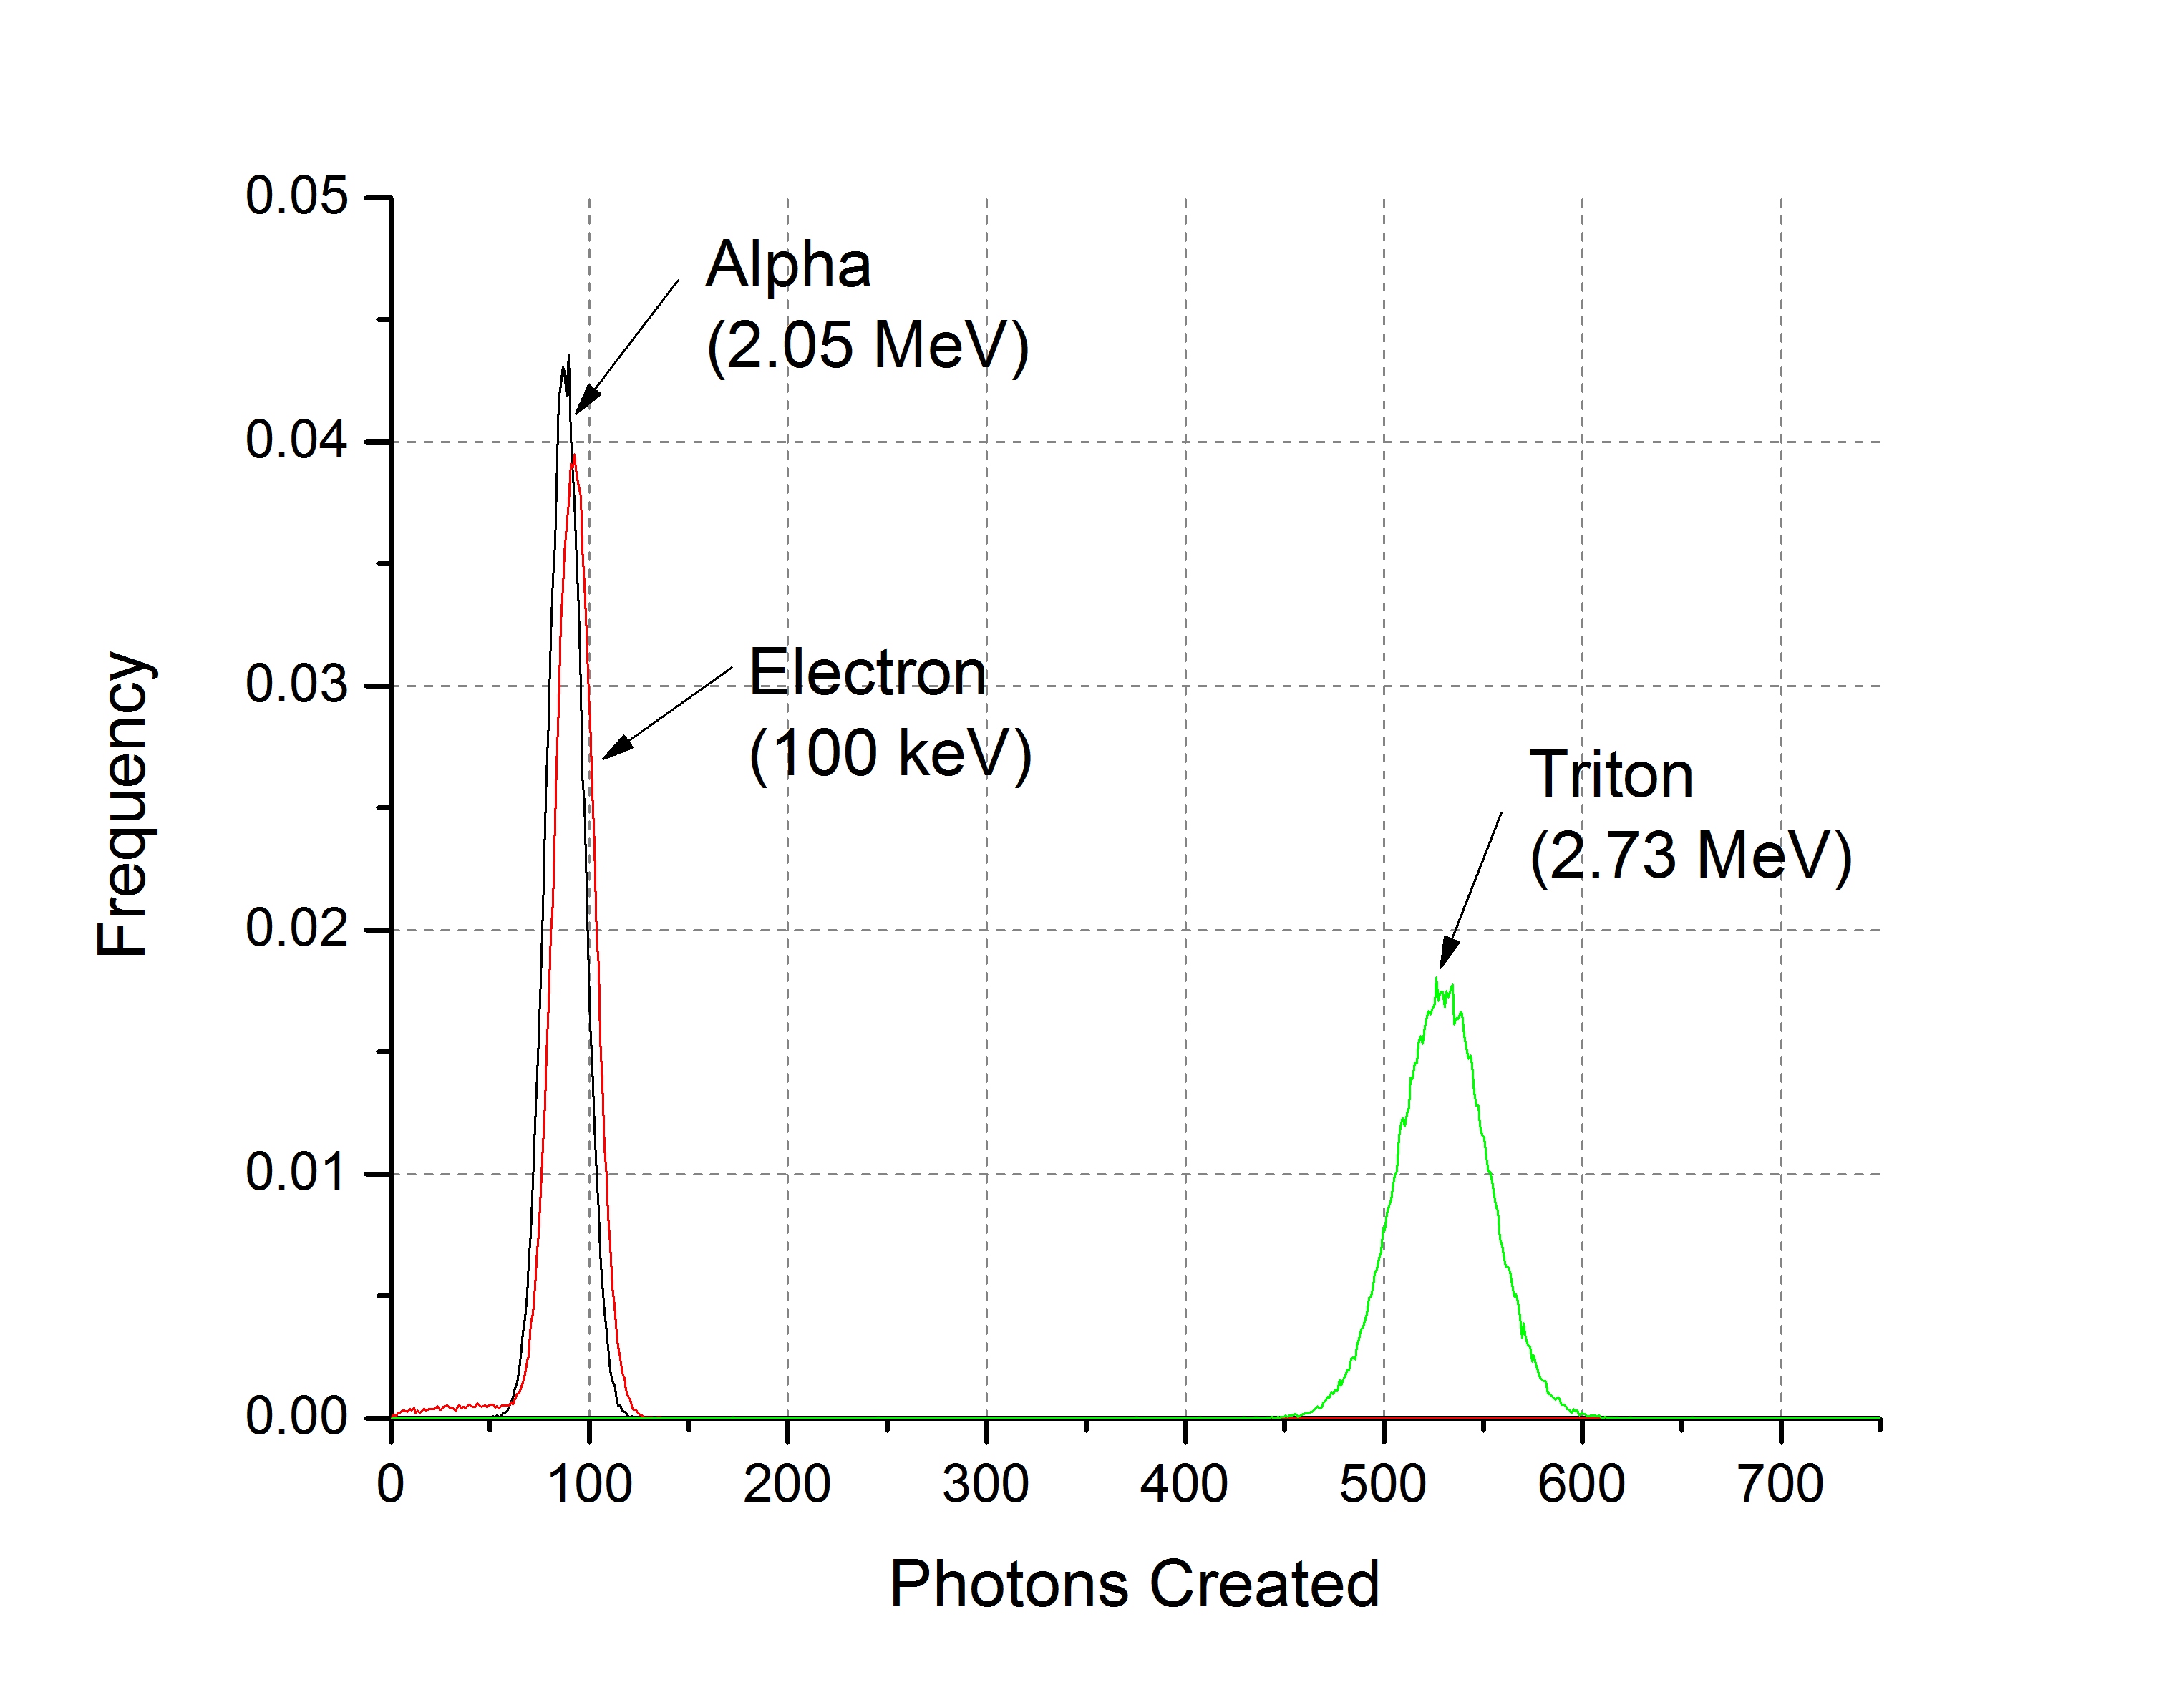
\includegraphics[width=\textwidth]{LightSim_AlphaTritonElectron}
    \caption{Simulated optical photons distributions for the particles of intrest in a portal monitor}
  \end{subfigure}
  \caption[Simulated Light Output of Alphas, Tritons, and Electrons]{GEANT4 simulated light output of alpha, tritons and electrons in polystryene. The light yield was assumed to be 1,000 photons per MeV.}
  \label{fig:SimLightOutputQuench}
\end{figure}

The pulse height deficit is computed by simulation of the charged particles and the corresponding electron.
This analysis yields a  pulse height deficit for the \iso[6]{Li} reaction as 8.5, and 27 for the \iso[10]{B}.
These results are summarized in \autoref{tab:PulseHeightDeficitSim}.
\begin{table}
  \caption[Simulated Number of Optical Photons for Selected Neutron Absorbitions]{GEANT4 simulated number of optical photons produced for the \iso[10]{B} and \iso[6]{Li} neutron absoribitions.  The sctintillator is assumed to have a light yeild of 1,000 photons per MeV}
  \label{tab:PulseHeightDeficitSim}
  \centering
  \begin{tabular}{c c c | c}
    \toprule
    & Particle & Photons Produced & Pulse Height Deficit \\
    \midrule
    \multirow{3}{*}{\iso[10]{B}} & $\alpha$ (\SI{1.78}{\MeV}) & 72 $\pm$ 8 &  \\
    & \iso[7]{Li} (\SI{1.02}{\MeV}) & 42 $\pm$ 8 & 27 \\
    & elctron (\SI{2.78}{\MeV}) & 3,030 $\pm$ 160 & \\
    \hline
    \multirow{3}{*}{\iso[6]{Li}} & $\alpha$ (\SI{2.05}{\MeV}) & 87 $\pm$ 9 & \\
    & triton (\SI{2.75}{\MeV}) & 528 $\pm$ 23 & 8.5\\
    & elctron (\SI{4.78}{\MeV}) & 5,250 $\pm$ 300 & \\
    \bottomrule
  \end{tabular}
\end{table}
